\documentclass[12pt]{article}
\usepackage{amsmath,amssymb,amsthm}
\usepackage{tikz}
\usepackage{float}
\usetikzlibrary{graphs,graphs.standard}
\usepackage{amsthm}
\usepackage{thmtools} % Much better for custom styles
% --- Custom Header Style to match your spacing ---
\makeatletter
\newtheoremstyle{mydef}
  {\topsep}   % Space above
  {\topsep}   % Space below
  {\normalfont} % Body font
  {}          % Indent amount
  {\bfseries} % Theorem head font
  {.}         % Punctuation after theorem head
  {\newline}  % We will handle the extra space in the head definition below
  {\thmname{#1}\thmnumber{ #2}\thmnote{ \bfseries #3}%
   \hfill\par\vspace{5pt}} % <--- This creates the break and the extra space
\makeatother
\theoremstyle{mydef}
\newtheorem{definition}{Definition}[section]
\newtheorem{theorem}{Theorem}[section]
\newtheorem{corollary}{Corollary}[section]
\newtheorem{problem}{Problem}[section]
\newtheorem{algorithm}{Algorithm}[section]
\usepackage{hyperref}
\hypersetup{
    colorlinks=true,
    linkcolor=blue,
    filecolor=magenta,      
    urlcolor=cyan,
}
\title{Chapter 1-4 --- Introduction to Graph Theory \\}
\author{Luca De Vecchis}
\date{Jan 2026}

\begin{document}
\maketitle
\tableofcontents
\newpage

\section{Graph Theory Basics}

\begin{definition}[Graph]

A \emph{graph} $G$ is an ordered pair
\[G = (V,E),\]
where $V$ is a finite nonempty set of \emph{vertices}, and $E$ is a finite multiset of unordered pairs of vertices called \emph{edges}. An edge may join two distinct vertices or a vertex to itself.
\end{definition}

\noindent Edges joining a vertex to itself are called \emph{loops}, and multiple edges are edges that join the same pair of vertices more than once.

\begin{definition}[Types of Graphs]
Different types of graphs include:
\begin{itemize}
    \item A \emph{simple graph} has no loops and no multiple edges.
    \item A \emph{multigraph} has no loops but may have multiple edges.
    \item A \emph{pseudograph} may have both loops and multiple edges.
\end{itemize}
\end{definition}

\subsubsection*{Examples}
\begin{figure}[h]
    \centering
    % --- Graph (a) K5 ---
    \begin{minipage}{0.3\textwidth}
        \centering
        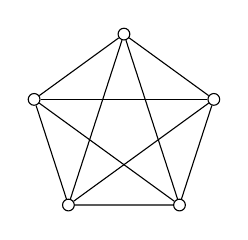
\begin{tikzpicture}[scale=0.8, vertex/.style={draw, circle, fill=white, inner sep=1.5pt}]
            \foreach \i in {1,...,5}
                \node[vertex] (v\i) at ({90 + (\i-1)*72}:1.5) {};
            \foreach \i in {1,...,5}
                \foreach \j in {\i,...,5}
                    \draw (v\i) -- (v\j);
        \end{tikzpicture}
        \\[0.2cm] (a)
    \end{minipage}
    \hfill
    % --- Graph (b) Cube ---
    \begin{minipage}{0.3\textwidth}
        \centering
        \begin{tikzpicture}[scale=0.8, vertex/.style={draw, circle, fill=white, inner sep=1.5pt}]
            \node[vertex] (o1) at (-1.5, -1.5) {};
            \node[vertex] (o2) at (1.5, -1.5) {};
            \node[vertex] (o3) at (1.5, 1.5) {};
            \node[vertex] (o4) at (-1.5, 1.5) {};
            \draw (o1) -- (o2) -- (o3) -- (o4) -- cycle;
            \node[vertex] (i1) at (-0.7, -0.7) {};
            \node[vertex] (i2) at (0.7, -0.7) {};
            \node[vertex] (i3) at (0.7, 0.7) {};
            \node[vertex] (i4) at (-0.7, 0.7) {};
            \draw (i1) -- (i2) -- (i3) -- (i4) -- cycle;
            \draw (o1) -- (i1); \draw (o2) -- (i2); \draw (o3) -- (i3); \draw (o4) -- (i4); \draw (o1) -- (o4); \draw (i1) -- (i4)
        \end{tikzpicture}
        \\[0.2cm] (b)
    \end{minipage}
    \hfill
    % --- Graph (c) K3,3 ---
    \begin{minipage}{0.3\textwidth}
        \centering
        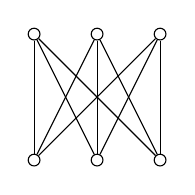
\begin{tikzpicture}[scale=0.8, vertex/.style={draw, circle, fill=white, inner sep=1.5pt}]
            \foreach \i in {1,2,3} \node[vertex] (u\i) at (\i, 2) {};
            \foreach \j in {1,2,3} \node[vertex] (v\j) at (\j, 0) {};
            \foreach \i in {1,2,3}
                \foreach \j in {1,2,3}
                    \draw (u\i) -- (v\j);
        \end{tikzpicture}
        \\[0.2cm] (c)
    \end{minipage}

    \vspace{0.5cm}
    \caption{(a) $K_5$; (b) the cube; (c) $K_{3,3}$}
\end{figure}

\begin{definition}[Order and Size]
The \emph{order} of a graph $G$ is $|V(G)|$, and the \emph{size} of $G$ is $|E(G)|$.
\end{definition}

\subsection{Graph Isomorphism}

\begin{definition}[Isomorphism]
Two graphs $G=(V,E)$ and $G'=(V',E')$ are \emph{isomorphic} if there exists a bijection
\[
\varphi: V \to V'
\]
such that for all $u,v \in V$,
\[
uv \in E \iff \varphi(u)\varphi(v) \in E'.
\]
\end{definition}

\begin{definition}[Isomorphism Invariants]
Quantities preserved under isomorphism include:
\begin{itemize}
    \item order and size,
    \item degree sequence,
    \item number of connected components,
    \item presence or absence of cycles.
\end{itemize}
\end{definition}

\subsection{Incidence and Adjacency Matrices}

Let $G$ be a graph with vertices $v_1,\dots,v_n$ and edges $e_1,\dots,e_m$.

\begin{definition}[Incidence Matrix]
The \emph{incidence matrix} $B=(b_{ij})$ of $G$ is
\[
b_{ij} =
\begin{cases}
1 & \text{if vertex } v_i \text{ is incident with edge } e_j,\\
0 & \text{otherwise}.
\end{cases}
\]
\end{definition}

\begin{definition}[Adjacency Matrix]
The \emph{adjacency matrix} $A=(a_{ij})$ of $G$ is
\[a_{ij} = \text{number of edges joining } v_i \text{ and } v_j.\]
For a simple graph, $A$ is symmetric and has zeros on the diagonal.
\end{definition}

\begin{figure}[H]
    \centering
    % --- Part 1: The Graph G ---
    \begin{minipage}{0.30\textwidth}
        \centering
        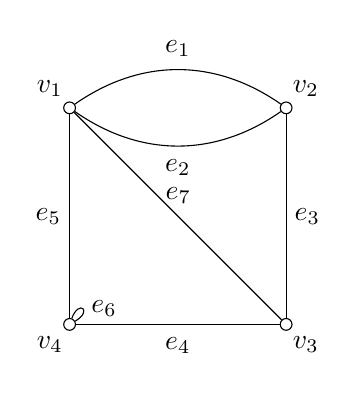
\begin{tikzpicture}[scale=1.1, every node/.style={circle, draw, inner sep=1.5pt, fill=white}]
            % Vertices
            \node (v1) at (0,2.5) [label=above left:$v_1$] {};
            \node (v2) at (2.5,2.5) [label=above right:$v_2$] {};
            \node (v3) at (2.5,0) [label=below right:$v_3$] {};
            \node (v4) at (0,0) [label=below left:$v_4$] {};

            % Edges
            \draw (v1) to[bend left=35] node[draw=none, fill=none, above] {$e_1$} (v2);
            \draw (v1) to[bend right=35] node[draw=none, fill=none, below] {$e_2$} (v2);
            \draw (v2) -- node[draw=none, fill=none, right] {$e_3$} (v3);
            \draw (v3) -- node[draw=none, fill=none, below] {$e_4$} (v4);
            \draw (v4) -- node[draw=none, fill=none, left] {$e_5$} (v1);
            \draw (v1) -- node[draw=none, fill=none, right, pos=0.4] {$e_7$} (v3);
            \draw (v4) to[out=30, in=70, looseness=12] node[draw=none, fill=none, right] {$e_6$} (v4);
        \end{tikzpicture}
        \\[0.3cm] $G$
    \end{minipage}
    \hfill
    % --- Part 2: Incidence Matrix M(G) ---
    \begin{minipage}{0.32\textwidth}
        \centering
        \setlength{\arraycolsep}{4pt} % Adjusts horizontal spacing in the matrix
        $\begin{array}{r|ccccccc}
              & e_1 & e_2 & e_3 & e_4 & e_5 & e_6 & e_7 \\ \hline
            v_1 & 1 & 1 & 0 & 0 & 1 & 0 & 1 \\
            v_2 & 1 & 1 & 1 & 0 & 0 & 0 & 0 \\
            v_3 & 0 & 0 & 1 & 1 & 0 & 0 & 1 \\
            v_4 & 0 & 0 & 0 & 1 & 1 & 2 & 0
        \end{array}$
        \\[0.3cm] $\mathbf{M}(G)$
    \end{minipage}
    \hfill
    % --- Part 3: Adjacency Matrix A(G) ---
    \begin{minipage}{0.28\textwidth}
        \centering
        \setlength{\arraycolsep}{5pt}
        $\begin{array}{r|cccc}
              & v_1 & v_2 & v_3 & v_4 \\ \hline
            v_1 & 0 & 2 & 1 & 1 \\
            v_2 & 2 & 0 & 1 & 0 \\
            v_3 & 1 & 1 & 0 & 1 \\
            v_4 & 1 & 0 & 1 & 1
        \end{array}$
        \\[0.3cm] $\mathbf{A}(G)$
    \end{minipage}

    \vspace{0.5cm}
    \caption{Incidence and Adjacency Matrix}
\end{figure}

\begin{theorem}[Walk Enumeration]
For a graph with adjacency matrix $A$, the $(i,j)$-entry of $A^k$ equals the number of walks of length $k$ from vertex $v_i$ to vertex $v_j$.
\end{theorem}

\subsection{Subgraphs}

\begin{definition}[Subgraph]
A graph $H$ is a \emph{subgraph} of $G$ if
\[V(H) \subseteq V(G), \quad E(H) \subseteq E(G),\]
with incidence preserved.
\end{definition}

\begin{definition}[Induced Subgraph]
For $S \subseteq V(G)$, the \emph{induced subgraph} $G[S]$ has vertex set $S$ and all edges of $G$ with both ends in $S$.
\end{definition}

\begin{definition}[Spanning Subgraph]
A subgraph $H$ of $G$ is \emph{spanning} if $V(H) = V(G)$.
\end{definition}

\begin{figure}[H]
    \centering
    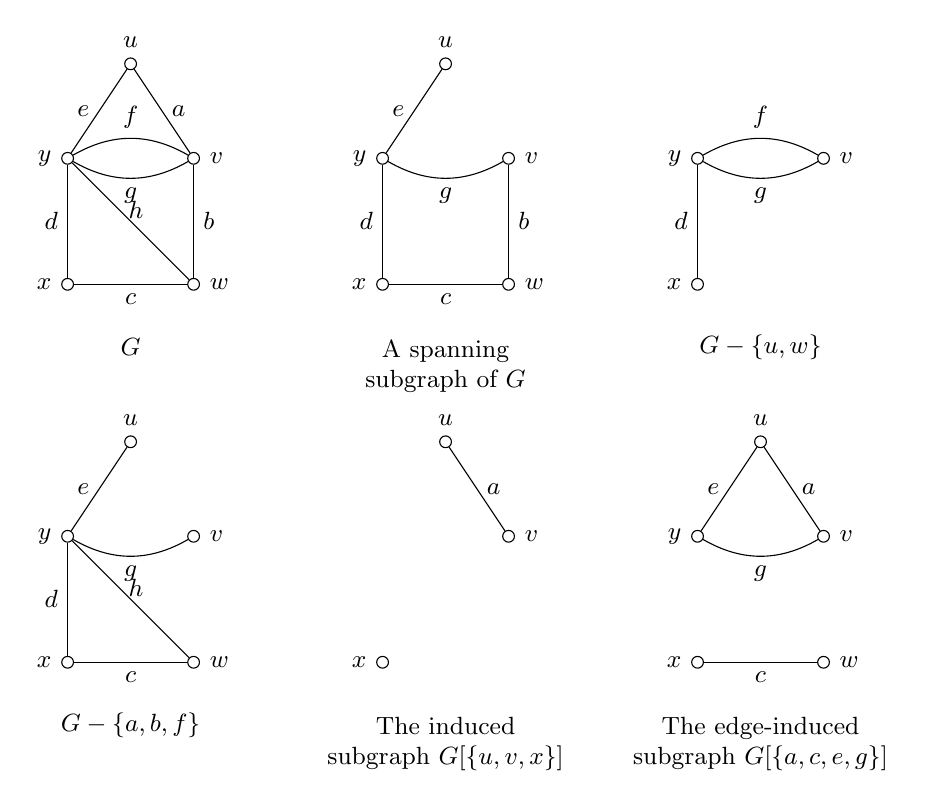
\begin{tikzpicture}[scale=0.8, vertex/.style={circle, draw, inner sep=1.5pt, fill=white}, every node/.style={font=\small}]
       
        % --- ROW 1 ---
        % (1) Graph G
        \begin{scope}[shift={(0,0)}]
            \node[vertex] (u) at (1,4) [label=above:$u$] {};
            \node[vertex] (y) at (0,2.5) [label=left:$y$] {};
            \node[vertex] (v) at (2,2.5) [label=right:$v$] {};
            \node[vertex] (x) at (0,0.5) [label=left:$x$] {};
            \node[vertex] (w) at (2,0.5) [label=right:$w$] {};
            
            \draw (u) -- node[left] {$e$} (y);
            \draw (u) -- node[right] {$a$} (v);
            \draw (y) to[bend left=30] node[above] {$f$} (v);
            \draw (y) to[bend right=30] node[below] {$g$} (v);
            \draw (y) -- node[left] {$d$} (x);
            \draw (y) -- node[right, pos=0.4] {$h$} (w);
            \draw (v) -- node[right] {$b$} (w);
            \draw (x) -- node[below] {$c$} (w);
            \node at (1,-0.5) {$G$};
        \end{scope}

        % (2) Spanning subgraph
        \begin{scope}[shift={(5,0)}]
            \node[vertex] (u) at (1,4) [label=above:$u$] {};
            \node[vertex] (y) at (0,2.5) [label=left:$y$] {};
            \node[vertex] (v) at (2,2.5) [label=right:$v$] {};
            \node[vertex] (x) at (0,0.5) [label=left:$x$] {};
            \node[vertex] (w) at (2,0.5) [label=right:$w$] {};
            
            \draw (u) -- node[left] {$e$} (y);
            \draw (y) to[bend right=30] node[below] {$g$} (v);
            \draw (y) -- node[left] {$d$} (x);
            \draw (v) -- node[right] {$b$} (w);
            \draw (x) -- node[below] {$c$} (w);
            \node[align=center] at (1,-0.8) {A spanning\\subgraph of $G$};
        \end{scope}

        % (3) G - {u, w}
        \begin{scope}[shift={(10,0)}]
            \node[vertex] (y) at (0,2.5) [label=left:$y$] {};
            \node[vertex] (v) at (2,2.5) [label=right:$v$] {};
            \node[vertex] (x) at (0,0.5) [label=left:$x$] {};
            
            \draw (y) to[bend left=30] node[above] {$f$} (v);
            \draw (y) to[bend right=30] node[below] {$g$} (v);
            \draw (y) -- node[left] {$d$} (x);
            \node at (1,-0.5) {$G - \{u, w\}$};
        \end{scope}

        % --- ROW 2 ---
        % (4) G - {a, b, f}
        \begin{scope}[shift={(0,-6)}]
            \node[vertex] (u) at (1,4) [label=above:$u$] {};
            \node[vertex] (y) at (0,2.5) [label=left:$y$] {};
            \node[vertex] (v) at (2,2.5) [label=right:$v$] {};
            \node[vertex] (x) at (0,0.5) [label=left:$x$] {};
            \node[vertex] (w) at (2,0.5) [label=right:$w$] {};
            
            \draw (u) -- node[left] {$e$} (y);
            \draw (y) to[bend right=30] node[below] {$g$} (v);
            \draw (y) -- node[left] {$d$} (x);
            \draw (y) -- node[right, pos=0.4] {$h$} (w);
            \draw (x) -- node[below] {$c$} (w);
            \node at (1,-0.5) {$G - \{a, b, f\}$};
        \end{scope}

        % (5) Induced subgraph G[{u, v, x}]
        \begin{scope}[shift={(5,-6)}]
            \node[vertex] (u) at (1,4) [label=above:$u$] {};
            \node[vertex] (v) at (2,2.5) [label=right:$v$] {};
            \node[vertex] (x) at (0,0.5) [label=left:$x$] {};
            
            \draw (u) -- node[right] {$a$} (v);
            \node[align=center] at (1,-0.8) {The induced\\subgraph $G[\{u, v, x\}]$};
        \end{scope}

        % (6) Edge-induced subgraph G[{a, c, e, g}]
        \begin{scope}[shift={(10,-6)}]
            \node[vertex] (u) at (1,4) [label=above:$u$] {};
            \node[vertex] (y) at (0,2.5) [label=left:$y$] {};
            \node[vertex] (v) at (2,2.5) [label=right:$v$] {};
            \node[vertex] (x) at (0,0.5) [label=left:$x$] {};
            \node[vertex] (w) at (2,0.5) [label=right:$w$] {};
            
            \draw (u) -- node[left] {$e$} (y);
            \draw (u) -- node[right] {$a$} (v);
            \draw (y) to[bend right=30] node[below] {$g$} (v);
            \draw (x) -- node[below] {$c$} (w);
            \node[align=center] at (1,-0.8) {The edge-induced\\subgraph $G[\{a, c, e, g\}]$};
        \end{scope}

    \end{tikzpicture}
    \vspace{0.5cm}
    \caption{Spanning and Induced Graphs}
\end{figure}

\subsection{Vertex Degrees}

\begin{definition}[Degree]
The \emph{degree} $d(v)$ of a vertex $v$ is the number of edges incident with $v$, with each loop counted twice.
\end{definition}

\begin{theorem}[Handshaking Lemma]
For any graph $G$,
\[
\sum_{v \in V(G)} d(v) = 2|E(G)|.
\]
\end{theorem}

\begin{corollary}
In any graph, the number of vertices with odd degree is even.
\end{corollary}

\subsection{Paths and Connectivity}

\begin{definition}[Walk, Trail, Path]
These are:
\begin{itemize}
    \item \emph{Walk}: sequence of vertices where consecutive vertices are adjacent.
    \item \emph{Trail}: walk with no repeated edges.
    \item \emph{Path}: walk with no repeated vertices.
\end{itemize}
\end{definition}

\begin{definition}[Connected Graph]
A graph is \emph{connected} if there is a path between every pair of vertices.
\end{definition}

\begin{theorem}
A graph is connected if and only if it contains a spanning tree.
\end{theorem}

\subsection{Cycles and Trees}

\begin{definition}[Cycle]
A \emph{cycle} is a closed path of length at least $3$ with no repeated vertices except the first and last.
\end{definition}

\begin{definition}[Tree]
A \emph{tree} is a connected graph containing no cycles.
\end{definition}

\begin{theorem}
A graph is acyclic if and only if it contains no cycles.
\end{theorem}
\clearpage

\subsection{Applications}
\subsubsection{Shortest Path Problem}

\begin{problem}[Shortest Path]
Given a connected graph with nonnegative edge weights, find a path of minimum total weight between two specified vertices.
\end{problem}

\begin{algorithm}[Dijkstra's Algorithm]
The steps are as it follows:
\begin{enumerate}
    \item Assign distance $0$ to the source vertex and $\infty$ to all others.
    \item Repeatedly select the unvisited vertex of minimum distance.
    \item Update distances to adjacent vertices via relaxation.
\end{enumerate}
\end{algorithm}

\noindent As the algorithm proceeds, these labels are modified so that, at the end of stage $i$,
\begin{equation*}
    l(u) = d(u_0, u) \quad \text{for} \quad u \in S_i
\end{equation*}
and
\begin{equation*}
    l(v) = \min_{u \in S_{i-1}} \{d(u_0, u) + w(uv)\} \quad \text{for} \quad v \in \bar{S}_i
\end{equation*}

\begin{figure}[H]
    \centering
    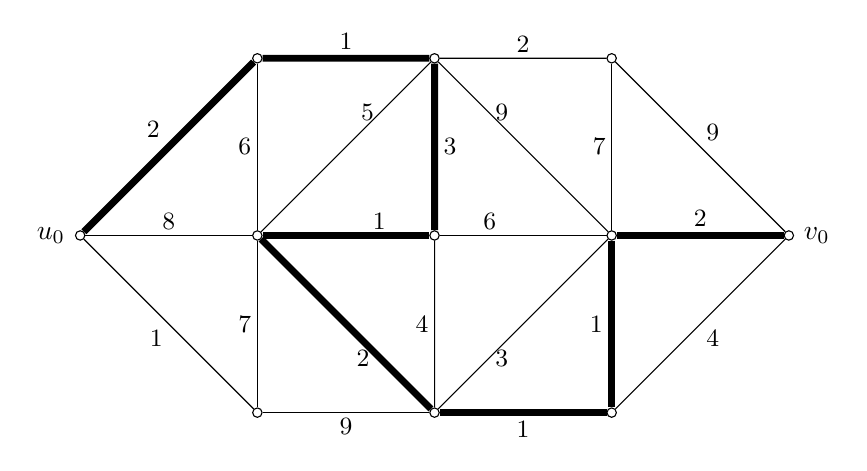
\begin{tikzpicture}[
        scale=1.5,
        vertex/.style={circle, draw, fill=white, inner sep=1.2pt},
        edge_label/.style={font=\small, inner sep=2pt},
        min_path/.style={line width=2.5pt} % Style for the bolded minimum weight path
    ]

    % --- Define Vertices ---
    \node[vertex] (u0) at (0,2) [label=left:$u_0$] {};
    
    % Column 1
    \node[vertex] (t1) at (1.5,3.5) {};
    \node[vertex] (m1) at (1.5,2) {};
    \node[vertex] (b1) at (1.5,0.5) {};
    
    % Column 2
    \node[vertex] (t2) at (3,3.5) {};
    \node[vertex] (m2) at (3,2) {};
    \node[vertex] (b2) at (3,0.5) {};
    
    % Column 3
    \node[vertex] (t3) at (4.5,3.5) {};
    \node[vertex] (m3) at (4.5,2) {};
    \node[vertex] (b3) at (4.5,0.5) {};
    
    \node[vertex] (v0) at (6,2) [label=right:$v_0$] {};

    % --- Draw Edges and Labels ---
    
    % From u0
    \draw[min_path] (u0) -- node[edge_label, above left] {2} (t1);
    \draw (u0) -- node[edge_label, above] {8} (m1);
    \draw (u0) -- node[edge_label, below left] {1} (b1);

    % Column 1 to Column 2
    \draw[min_path] (t1) -- node[edge_label, above] {1} (t2);
    \draw (m1) -- node[edge_label, above, pos=0.7] {1} (m2);
    \draw (b1) -- node[edge_label, below] {9} (b2);
    \draw (m1) -- node[edge_label, left, pos=0.7] {5} (t2);
    \draw[min_path] (m1) -- node[edge_label, below, pos=0.6] {2} (b2);
    
    % Column 2 to Column 3
    \draw (t2) -- node[edge_label, above] {2} (t3);
    \draw (m2) -- node[edge_label, above, pos=0.3] {6} (m3);
    \draw[min_path] (b2) -- node[edge_label, below] {1} (b3);
    \draw (t2) -- node[edge_label, right, pos=0.3] {9} (m3);
    \draw (b2) -- node[edge_label, right, pos=0.3] {3} (m3);

    % Column 3 to v0
    \draw (t3) -- node[edge_label, above right] {9} (v0);
    \draw[min_path] (m3) -- node[edge_label, above] {2} (v0);
    \draw (b3) -- node[edge_label, below right] {4} (v0);

    % Vertical Edges
    \draw (t1) -- node[edge_label, left] {6} (m1);
    \draw (m1) -- node[edge_label, left] {7} (b1);
    
    % Bolded horizontal 1 from Column 2 to Column 1 (m2 to m1)
    \draw[min_path] (m2) -- (m1);
    
    \draw[min_path] (t2) -- node[edge_label, right] {3} (m2);
    \draw (m2) -- node[edge_label, left] {4} (b2);
    
    \draw (t3) -- node[edge_label, left] {7} (m3);
    \draw[min_path] (m3) -- node[edge_label, left] {1} (b3);

    \end{tikzpicture}
    \vspace{0.5cm}
    \caption{A $(u_0, v_0)$-path of minimum weight}
\end{figure}

\subsection{Sperner's Lemma}

\begin{theorem}[Sperner's Lemma]
Let a triangle be subdivided into smaller triangles with vertices labeled $\{1,2,3\}$ such that boundary vertices satisfy the Sperner labeling conditions. Then there exists at least one subtriangle whose vertices have all three labels.
\end{theorem}

\begin{figure}[H]
    \centering
    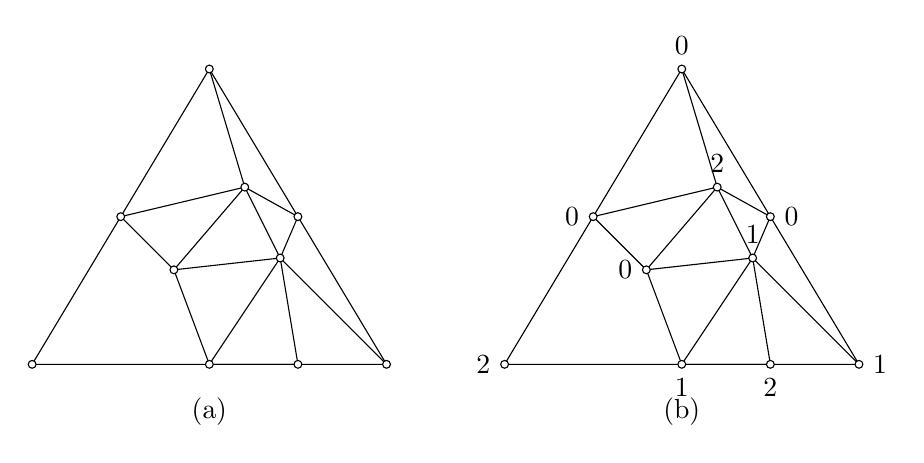
\begin{tikzpicture}[scale=1.5, vertex/.style={circle, draw, fill=white, inner sep=1pt}]

        % --- (a) Simplicial Subdivision ---
        \begin{scope}[shift={(0,0)}]
            % Outer Triangle Vertices
            \coordinate (A) at (0,0);
            \coordinate (B) at (3,0);
            \coordinate (C) at (1.5,2.5);

            % Boundary subdivision points
            \coordinate (AB1) at (1.5,0);
            \coordinate (AB2) at (2.25,0);
            \coordinate (BC1) at (2.25,1.25);
            \coordinate (AC1) at (0.75,1.25);

            % Interior points
            \coordinate (I1) at (1.2,0.8);
            \coordinate (I2) at (1.8,1.5);
            \coordinate (I3) at (2.1,0.9);

            % Draw edges
            \draw (A) -- (B) -- (C) -- cycle;
            \draw (AC1) -- (I1) -- (AB1);
            \draw (I1) -- (I2) -- (AC1);
            \draw (I2) -- (BC1) -- (I3) -- (I2);
            \draw (I3) -- (AB2) -- (AB1) -- (I3);
            \draw (I1) -- (I3);
            \draw (C) -- (I2);
            \draw (B) -- (I3);

            % Vertices
            \foreach \p in {A,B,C,AB1,AB2,BC1,AC1,I1,I2,I3}
                \node[vertex] at (\p) {};

            \node at (1.5,-0.4) {(a)};
        \end{scope}

        % --- (b) Proper Labelling ---
        \begin{scope}[shift={(4,0)}]
            % Coordinates (same as above)
            \coordinate (A2) at (0,0);
            \coordinate (B2) at (3,0);
            \coordinate (C2) at (1.5,2.5);
            \coordinate (AB1_2) at (1.5,0);
            \coordinate (AB2_2) at (2.25,0);
            \coordinate (BC1_2) at (2.25,1.25);
            \coordinate (AC1_2) at (0.75,1.25);
            \coordinate (I1_2) at (1.2,0.8);
            \coordinate (I2_2) at (1.8,1.5);
            \coordinate (I3_2) at (2.1,0.9);

            % Draw edges
            \draw (A2) -- (B2) -- (C2) -- cycle;
            \draw (AC1_2) -- (I1_2) -- (AB1_2);
            \draw (I1_2) -- (I2_2) -- (AC1_2);
            \draw (I2_2) -- (BC1_2) -- (I3_2) -- (I2_2);
            \draw (I3_2) -- (AB2_2) -- (AB1_2) -- (I3_2);
            \draw (I1_2) -- (I3_2);
            \draw (C2) -- (I2_2);
            \draw (B2) -- (I3_2);

            % Vertices with labels matching the image
            \node[vertex, label=left:2] at (A2) {};
            \node[vertex, label=right:1] at (B2) {};
            \node[vertex, label=above:0] at (C2) {};
            
            \node[vertex, label=below:1] at (AB1_2) {};
            \node[vertex, label=below:2] at (AB2_2) {};
            \node[vertex, label=right:0] at (BC1_2) {};
            \node[vertex, label=left:0] at (AC1_2) {};
            
            \node[vertex, label=left:0] at (I1_2) {};
            \node[vertex, label=above:2] at (I2_2) {};
            \node[vertex, label=above:1] at (I3_2) {};

            \node at (1.5,-0.4) {(b)};
        \end{scope}

    \end{tikzpicture}
    \vspace{0.5cm}
    \caption{(a) A simplicial subdivision of a triangle; (b) a proper labelling of the subdivision}
\end{figure}

\section{Trees}

\subsection{Trees}

\begin{definition}[Tree]
A \emph{tree} is a connected graph containing no cycles.
Trees are the fundamental acyclic connected structures in graph theory and play a central role in both theory and applications.
\end{definition}

\begin{figure}[H]
    \centering
    \begin{tikzpicture}[
        scale=0.8, 
        vertex/.style={circle, draw, fill=white, inner sep=1.2pt},
        edge/.style={thick}
    ]

    % --- 1. Path Graph P6 ---
    \begin{scope}[shift={(0,0)}]
        \foreach \i in {1,...,6}
            \node[vertex] (v\i) at (0, \i) {};
        \foreach \i [evaluate=\i as \j using int(\i+1)] in {1,...,5}
            \draw[edge] (v\i) -- (v\j);
    \end{scope}

    % --- 2. Tree with one branch ---
    \begin{scope}[shift={(2.5,0)}]
        \foreach \i in {1,...,4} \node[vertex] (v\i) at (0, \i+1) {};
        \node[vertex] (v5) at (-0.6, 1) {};
        \node[vertex] (v6) at (0.6, 1) {};
        \draw[edge] (v1) -- (v2) -- (v3) -- (v4);
        \draw[edge] (v5) -- (v1) -- (v6);
    \end{scope}

    % --- 3. Y-shaped Tree ---
    \begin{scope}[shift={(5,0)}]
        \foreach \i in {1,2,3} \node[vertex] (v\i) at (0, \i+2) {};
        \node[vertex] (v4) at (0, 3) {};
        \node[vertex] (v5) at (-0.8, 1) {};
        \node[vertex] (v6) at (0.8, 1) {};
        \draw[edge] (v1) -- (v2) -- (v3);
        \draw[edge] (v5) -- (v4) -- (v6);
        \draw[edge] (v4) -- (v1);
    \end{scope}

    % --- 4. Tree with 3-leaf star at bottom ---
    \begin{scope}[shift={(7.5,0)}]
        \foreach \i in {1,...,3} \node[vertex] (v\i) at (0, \i+1.5) {};
        \node[vertex] (v4) at (-0.7, 1) {};
        \node[vertex] (v5) at (0, 1) {};
        \node[vertex] (v6) at (0.7, 1) {};
        \draw[edge] (v1) -- (v2) -- (v3);
        \draw[edge] (v4) -- (v1);
        \draw[edge] (v5) -- (v1);
        \draw[edge] (v6) -- (v1);
    \end{scope}

    % --- 5. Double-Y Tree ---
    \begin{scope}[shift={(10,0)}]
        \node[vertex] (c1) at (0, 3);
        \node[vertex] (c2) at (0, 2);
        \node[vertex] (v1) at (-0.7, 4);
        \node[vertex] (v2) at (0.7, 4);
        \node[vertex] (v3) at (-0.7, 1);
        \node[vertex] (v4) at (0.7, 1) {};
        \draw[edge] (c1) -- (c2);
        \draw[edge] (v1) -- (c1) -- (v2);
        \draw[edge] (v3) -- (c2) -- (v4);
    \end{scope}

    % --- 6. Star Graph S6 ---
    \begin{scope}[shift={(12.5,2)}]
        \node[vertex] (center) at (0,0) {};
        \foreach \i in {1,...,5}
            \node[vertex] (v\i) at ({18 + (\i-1)*72}:1.2) {};
        \foreach \i in {1,...,5}
            \draw[edge] (center) -- (v\i);
    \end{scope}

    \end{tikzpicture}
    \vspace{0.5cm}
    \caption{The trees on six vertices}
\end{figure}

\begin{theorem}[Equivalent Characterizations of Trees]

Let $G$ be a graph with $n$ vertices. The following statements are equivalent:

\begin{enumerate}
    \item $G$ is a tree.
    \item $G$ is connected and has $n-1$ edges.
    \item $G$ is acyclic and has $n-1$ edges.
    \item $G$ is connected, and the removal of any edge disconnects $G$.
    \item $G$ is acyclic, and the addition of any edge creates exactly one cycle.
    \item There is a unique path between every pair of vertices of $G$.
\end{enumerate}
\end{theorem}

\noindent \textbf{Corollary 2.2} Every nontrivial tree has at least two vertices of degree one.

\vspace{0.3cm}

\noindent \textit{Proof} Let $G$ be a nontrivial tree. Then:
\begin{equation*}
    d(v) \geq 1 \quad \text{for all} \quad v \in V
\end{equation*}
Also, by theorems 1.1 and 2.2, we have
\begin{equation*}
    \sum_{v \in V} d(v) = 2\varepsilon = 2\nu - 2
\end{equation*}
It now follows that $d(v) = 1$ for at least two vertices $v$. \hfill

\clearpage

\subsection{Cut Edges and Bonds}

\begin{definition}[Cut Edge (Bridge)]

An edge $e$ of a graph $G$ is a \emph{cut edge} if $G - e$ has more connected components than $G$.
\end{definition}

\begin{theorem}
An edge of a graph is a cut edge if and only if it lies on no cycle.
\end{theorem}

\begin{corollary}
Every edge of a tree is a cut edge.
\end{corollary}

\begin{definition}[Bond]
A \emph{bond} is a minimal nonempty set of edges whose deletion increases the number of connected components of the graph.
\end{definition}


\subsection{Cut Vertices}

\begin{definition}[Cut Vertex (Articulation Point)]
A vertex $v$ of a graph $G$ is a \emph{cut vertex} if $G - v$ has more connected components than $G$.
\end{definition}

\begin{theorem}
A vertex $v$ is a cut vertex if and only if there exist vertices $x,y \neq v$ such that every $x$--$y$ path passes through $v$.\\
In a path $P_n$ with $n \geq 3$, all internal vertices are cut vertices, while endpoints are not.
\end{theorem}

\subsection{Cayley's Formula}

\begin{theorem}[Cayley's Formula]

The number of distinct labeled trees on $n$ vertices is
\[n^{\,n-2}.\]
For $n=3$, there are $3^1 = 3$ labeled trees.  
For $n=4$, there are $4^2 = 16$ labeled trees.
\end{theorem}

\begin{figure}[H]
    \centering
    \begin{tikzpicture}[
        scale=1.2,
        vertex/.style={circle, draw, fill=white, inner sep=1.2pt},
        every node/.style={font=\small}
    ]

    % --- Left Graph: G ---
    \begin{scope}[shift={(0,0)}]
        % Vertices
        \node[vertex] (v1) at (0,3) [label=above:$v_1$] {};
        \node[vertex] (v2) at (3,3) [label=above:$v_2$] {};
        \node[vertex] (v3) at (3,0) [label=right:$v_3$] {};
        \node[vertex] (v4) at (0,0) [label=left:$v_4$] {};

        % Edges
        \draw (v1) -- node[above] {$e_1$} (v2);
        \draw (v2) -- node[right] {$e_2$} (v3);
        \draw (v3) -- node[below] {$e_3$} (v4);
        \draw (v4) -- node[left] {$e_4$} (v1);
        \draw (v1) -- node[above right, pos=0.4] {$e$} (v3);

        \node at (1.5,-0.8) {$G$};
    \end{scope}

    % --- Transformation Arrow ---
    \draw[thick, ->] (4,1.5) -- (5.5,1.5);

    % --- Right Graph: G . e ---
    \begin{scope}[shift={(7,0)}]
        % Vertices
        \node[vertex] (v1v3) at (1,1.5) [label=right:{$\{v_1, v_3\}$}] {};
        \node[vertex] (v2) at (2.5,3) [label=above:$v_2$] {};
        \node[vertex] (v4) at (-0.5,0) [label=below:$v_4$] {};

        % Arched Edges (multi-edges)
        \draw (v1v3) to[bend left=25] node[above left] {$e_1$} (v2);
        \draw (v1v3) to[bend right=25] node[below right] {$e_2$} (v2);
        
        \draw (v1v3) to[bend right=25] node[above left] {$e_4$} (v4);
        \draw (v1v3) to[bend left=25] node[below right] {$e_3$} (v4);

        \node at (1,-0.8) {$G \cdot e$};
    \end{scope}

    \end{tikzpicture}
    \vspace{0.5cm}
    \caption{Contraction of an edge}
\end{figure}

\subsubsection*{Proof Idea (Prüfer Codes)}

Each labeled tree on $n$ vertices corresponds uniquely to a Prüfer sequence of length $n-2$, with entries in $\{1,\dots,n\}$. This gives a bijection between labeled trees and sequences of length $n-2$ over $n$ elements.

\subsection{Applications}

\subsubsection{Spanning Trees}

\begin{definition}[Spanning Tree]

A \emph{spanning tree} of a connected graph $G$ is a spanning subgraph of $G$ that is a tree.
\end{definition}

\begin{theorem}
Every connected graph has at least one spanning tree.\\
Removing one edge from each cycle of a connected graph produces a spanning tree.
\end{theorem}

\clearpage

\subsubsection{Minimum Spanning Trees}

\begin{problem}[Minimum Spanning Tree]
Given a connected graph with edge weights, find a spanning tree of minimum total weight.
\end{problem}

\begin{algorithm}[Kruskal's Algorithm]
The steps are as follows:
\begin{enumerate}
    \item Sort edges in nondecreasing order of weight.
    \item Add edges one by one, skipping those that create a cycle.
    \item Stop when $n-1$ edges have been selected.
\end{enumerate}
\end{algorithm}

\begin{algorithm}[Prim's Algorithm]
The steps are as follows:
\begin{enumerate}
    \item Start with a single vertex.
    \item Repeatedly add the minimum-weight edge joining the tree to a new vertex.
\end{enumerate}
\end{algorithm}

\begin{theorem}
Both Kruskal's and Prim's algorithms produce a minimum spanning tree.
\end{theorem}

\begin{figure}[H]
    \centering
    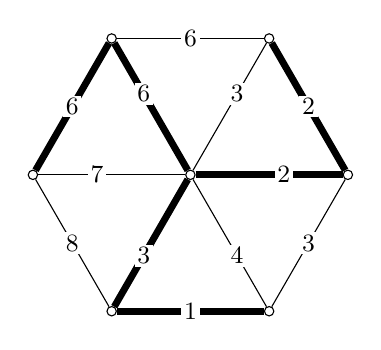
\begin{tikzpicture}[
        scale=2,
        vertex/.style={circle, draw, fill=white, inner sep=1.2pt},
        edge_label/.style={font=\small, fill=white, inner sep=1pt},
        optimal/.style={line width=2.5pt} % Bold style for the optimal tree
    ]

    % --- Define Vertices ---
    \node[vertex] (center) at (0,0) {};
    
    % Surrounding vertices in a hexagon (starting from top left)
    \node[vertex] (v1) at (120:1) {};
    \node[vertex] (v2) at (60:1) {};
    \node[vertex] (v3) at (0:1) {};
    \node[vertex] (v4) at (300:1) {};
    \node[vertex] (v5) at (240:1) {};
    \node[vertex] (v6) at (180:1) {};

    % --- Draw Edges and Weights ---
    
    % Outer Hexagon Edges
    \draw (v1) -- node[edge_label] {6} (v2);
    \draw[optimal] (v2) -- node[edge_label] {2} (v3);
    \draw (v3) -- node[edge_label] {3} (v4);
    \draw[optimal] (v4) -- node[edge_label] {1} (v5);
    \draw (v5) -- node[edge_label] {8} (v6);
    \draw[optimal] (v6) -- node[edge_label] {6} (v1);

    % Spokes (Internal Edges)
    \draw[optimal] (center) -- node[edge_label, pos=0.6] {6} (v1);
    \draw (center) -- node[edge_label, pos=0.6] {3} (v2);
    \draw[optimal] (center) -- node[edge_label, pos=0.6] {2} (v3);
    \draw (center) -- node[edge_label, pos=0.6] {4} (v4);
    \draw[optimal] (center) -- node[edge_label, pos=0.6] {3} (v5);
    \draw (center) -- node[edge_label, pos=0.6] {7} (v6);

    \end{tikzpicture}
    \vspace{0.5cm}
    \caption{An optimal tree in a weighted graph}
\end{figure}

\clearpage

\subsection{The Connector Problem}

\begin{problem}[Connector Problem]

Given a connected graph with weighted edges, find a minimum-weight set of edges that keeps the graph connected.
\end{problem}

\begin{theorem}
The solution to the connector problem is a minimum spanning tree.\\
Designing a minimum-cost communication or road network that connects all locations without redundancy is an instance of the connector problem.
\end{theorem}

\subsection{Structural Properties of Trees}

\begin{theorem}

Every tree with at least two vertices has at least two vertices of degree $1$.
\end{theorem}

\noindent\textit{Proof Sketch.}
Assume all vertices have degree at least $2$. Then the sum of degrees is at least $2n$, contradicting the handshaking lemma for a tree with $n-1$ edges.

\begin{corollary}
Every tree can be constructed by successively attaching leaves.
\end{corollary}

\subsection{Summary of Chapter 2}

\begin{itemize}
    \item Trees are connected acyclic graphs.
    \item They have exactly $n-1$ edges.
    \item Every edge of a tree is a cut edge.
    \item Cayley's formula counts labeled trees.
    \item Spanning trees connect general graphs to tree theory.
    \item Minimum spanning trees solve optimization problems on networks.
\end{itemize}

\section{Connectivity}

\subsection{Definitions of Connectivity}

\begin{definition}[Vertex Cut]
Let $G = (V, E)$ be a graph. A subset $S \subset V$ is a \emph{vertex cut} (or separating set) if the induced subgraph $G - S$ is disconnected or contains only a single vertex.
\end{definition}

\begin{definition}[Vertex-Connectivity]
The \emph{vertex-connectivity} of a graph $G$, denoted by $\kappa(G)$, is the minimum number of vertices whose removal disconnects $G$ or leaves a trivial graph. 
\begin{itemize}
    \item For a non-complete graph, $\kappa(G)$ is the size of the smallest vertex cut.
    \item For a complete graph $K_n$, we define $\kappa(K_n) = n - 1$.
\end{itemize}
\end{definition}

\begin{definition}[Edge Cut]
A subset of edges $F \subseteq E(G)$ is an \emph{edge cut} if $G - F$ has more connected components than $G$.
\end{definition}

\begin{definition}[Edge-Connectivity]
The \emph{edge-connectivity} of $G$, denoted by $\lambda(G)$, is the minimum size of an edge cut. If $G$ is disconnected or has only one vertex, $\lambda(G) = 0$.
\end{definition}

\begin{definition}[$k$-Connectedness]
A graph $G$ is said to be:
\begin{itemize}
    \item \textbf{$k$-connected} if $\kappa(G) \ge k$. This implies the graph remains connected after removing any $k-1$ vertices.
    \item \textbf{$k$-edge-connected} if $\lambda(G) \ge k$. This implies the graph remains connected after removing any $k-1$ edges.
\end{itemize}
\end{definition}

\subsection{Fundamental Inequalities}

\begin{theorem}[Whitney, 1932]
For any nontrivial graph $G$, the following relationship holds:
\[ \kappa(G) \le \lambda(G) \le \delta(G) \]
where $\delta(G)$ represents the minimum degree of the vertices in $G$.
\end{theorem}

\noindent \textit{Proof Sketch}
1. To show $\lambda(G) \le \delta(G)$: Let $v$ be a vertex with $deg(v) = \delta(G)$. Deleting all edges incident to $v$ isolates $v$, thus disconnecting the graph using exactly $\delta(G)$ edges.
2. To show $\kappa(G) \le \lambda(G)$: Removing one endpoint from each edge in a minimum edge cut creates a vertex set that disconnects the graph (though technical care is needed for cases where edges share endpoints).

\subsubsection{The Cycle Graph $C_n$}
For any cycle $C_n$ where $n \ge 3$:
\begin{itemize}
    \item $\delta(C_n) = 2$ (each vertex has two neighbors).
    \item $\lambda(C_n) = 2$ (cutting one edge leaves a path; cutting two edges disconnects it).
    \item $\kappa(C_n) = 2$ (removing one vertex leaves a path; removing two disconnects it).
\end{itemize}
\[ \kappa(C_n) = \lambda(C_n) = \delta(C_n) = 2 \]

\begin{center}
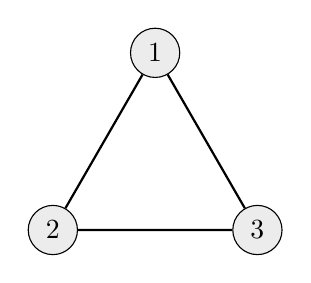
\begin{tikzpicture}[scale=1, every node/.style={circle,draw,inner sep=1.2mm, fill=lightgray!30}]
\node (1) at (90:1.5) {1};
\node (2) at (210:1.5) {2};
\node (3) at (330:1.5) {3};
\draw[thick] (1) -- (2) -- (3) -- (1);
\end{tikzpicture}
\end{center}

\subsection{Vertex Cuts and Separating Sets}

\begin{definition}[Separating Set]
While any set $S$ that disconnects $G$ is a vertex cut, a \emph{separating set} is specifically a vertex cut of minimum cardinality $\kappa(G)$. 
\end{definition}

\begin{theorem}
A connected graph $G$ with at least three vertices is $2$-connected if and only if it contains no \emph{cut vertices} (also known as articulation points). 
\end{theorem}

\noindent \textbf{Path $P_n$ vs. Cycle $C_n$}\\
In a path $P_n$ ($n \ge 3$), any "inner" vertex is a cut vertex because its removal splits the path into two or more components. Consequently, $\kappa(P_n) = 1$, making it $1$-connected but not $2$-connected.

\begin{figure}[H]
    \centering
    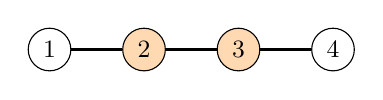
\begin{tikzpicture}[scale=1.2, every node/.style={circle,draw,inner sep=1mm, font=\small}]
    % Path P4
    \node (1) at (0,0) {1};
    \node[fill=orange!30] (2) at (1,0) {2};
    \node[fill=orange!30] (3) at (2,0) {3};
    \node (4) at (3,0) {4};
    \draw[thick] (1) -- (2) -- (3) -- (4);
    \end{tikzpicture}
        \vspace{0.2cm}
        \caption{$P_4$: Orange nodes are cut-vertices}
\end{figure}

\subsection{Menger's Theorem (Vertex Version)}

Menger's Theorem is a cornerstone of network reliability. It establishes a "min-max" relationship: the difficulty of disconnecting two points is exactly equal to the number of independent "highways" between them.

\begin{definition}[Internally Disjoint Paths]
Two $x,y$-paths are \emph{internally disjoint} if they do not share any vertices other than the start ($x$) and the end ($y$). These represent parallel routes that do not rely on the same intermediate "hubs."
\end{definition}

\begin{theorem}[Menger's Theorem — Vertex Form]
Let $x$ and $y$ be distinct nonadjacent vertices of $G$. The maximum number of pairwise internally disjoint $x,y$-paths equals the minimum number of vertices whose removal separates $x$ from $y$.
\end{theorem}

\begin{corollary}
A graph $G$ is $k$-connected if and only if every pair of vertices has at least $k$ internally disjoint paths between them.
\end{corollary}

%========================
% Improved TikZ: Menger's Paths
%========================
\begin{figure}[H]
    \centering
    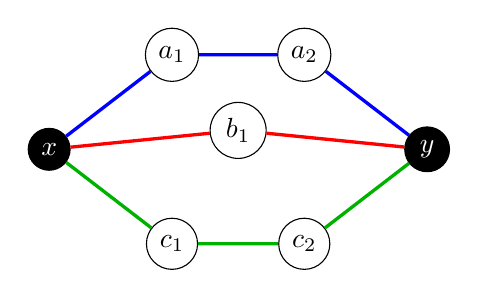
\begin{tikzpicture}[scale=1.2, every node/.style={circle,draw,inner sep=1mm}]
    \node[fill=black, text=white] (x) at (0,0) {$x$};
    \node[fill=black, text=white] (y) at (4,0) {$y$};
    
    % Path 1
    \node (a1) at (1.3, 1) {$a_1$};
    \node (a2) at (2.7, 1) {$a_2$};
    \draw[very thick, blue] (x) -- (a1) -- (a2) -- (y);
    
    % Path 2
    \node (b1) at (2, 0.2) {$b_1$};
    \draw[very thick, red] (x) -- (b1) -- (y);
    
    % Path 3
    \node (c1) at (1.3, -1) {$c_1$};
    \node (c2) at (2.7, -1) {$c_2$};
    \draw[very thick, green!70!black] (x) -- (c1) -- (c2) -- (y);

    \end{tikzpicture}
    \vspace{0.2cm}
        \caption{\small Three internally disjoint paths $\implies$ 3-connected locally}
\end{figure}

\subsection{Blocks and Decomposition}

\begin{definition}[Block]
A \emph{block} (or biconnected component) of a graph $G$ is a maximal subgraph such that any two vertices in the block can be connected by at least two internally disjoint paths. 
\end{definition}

In practical terms, a block is either:
\begin{itemize}
    \item A bridge (a single edge that, if removed, disconnects the graph).
    \item A maximal $2$-connected subgraph (like a cycle or a complex cluster).
\end{itemize}

\begin{theorem}[Block Decomposition]
Any connected graph $G$ is the union of its blocks. While edges belong to exactly one block, vertices can belong to multiple blocks. A vertex belongs to more than one block if and only if it is a \emph{cut vertex}.
\end{theorem}

\noindent \textbf{Tree Decomposition}\\ 
In a tree, every single edge is its own block. The cut vertices are all nodes with a degree $> 1$.

\begin{figure}[H]
    \centering
    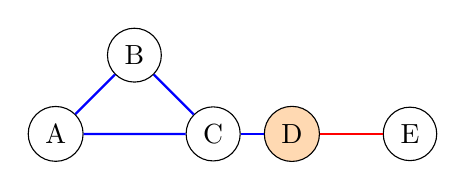
\begin{tikzpicture}[scale=1, every node/.style={circle,draw,inner sep=1.2mm}]
    % Original Graph with a Cycle and a "Tail"
    \node (A) at (0,0) {A};
    \node (B) at (1,1) {B};
    \node (C) at (2,0) {C};
    \node[fill=orange!30] (D) at (3,0) {D}; % Cut vertex
    \node (E) at (4.5,0) {E};
    
    \draw[thick, blue] (A) -- (B) -- (C) -- (A); % Block 1 (Cycle)
    \draw[thick, red] (D) -- (E);                % Block 2 (Bridge)
    \draw[thick, blue] (C) -- (D);               % Part of Block 1 (if 2-conn) or separate
    \end{tikzpicture}
    \vspace{0.2cm}
        \caption{\small Vertex D is the "hinge" between two blocks.}
\end{figure}

\subsection{The Block-Cut Tree}

\begin{definition}[Block-Cut Tree]
The structure of how blocks are connected can be represented by a \emph{Block-Cut Tree} (or Block Graph). This is a bipartite graph where:
\begin{itemize}
    \item One set of nodes represents the \textbf{Blocks} ($B_1, B_2, \dots$).
    \item The other set represents the \textbf{Cut Vertices} ($v_1, v_2, \dots$).
    \item An edge exists between a block node and a cut vertex node if the vertex belongs to that block in the original graph.
\end{itemize}
\end{definition}

\subsection{Applications: Network Reliability}

In network design, connectivity is a proxy for \textbf{fault tolerance}. 

\begin{itemize}
    \item \textbf{Vertex-Connectivity ($\kappa$):} Measures resistance to node failure (e.g., a router crashing).
    \item \textbf{Edge-Connectivity ($\lambda$):} Measures resistance to link failure (e.g., a fiber cable being cut).
\end{itemize}

\subsubsection{Comparison of Topologies}
Consider a network with $n$ nodes:
\begin{table}[h]
\centering
\begin{tabular}{lcccc}
\hline
\textbf{Topology} & $\kappa(G)$ & $\lambda(G)$ & \textbf{Reliability} & \textbf{Cost (Edges)} \\ \hline
Path ($P_n$) & 1 & 1 & Very Low & $n-1$ \\
Cycle ($C_n$) & 2 & 2 & Medium & $n$ \\
Complete ($K_n$) & $n-1$ & $n-1$ & Extremely High & $n(n-1)/2$ \\ \hline
\end{tabular}
\end{table}
\clearpage

\subsection{Harary Graphs and Minimum Edges}

We denote by $f(m, n)$ the minimum number of edges that an $m$-connected graph on $n$ vertices can have (where $m < n$). According to the relationship between connectivity and minimum degree ($\kappa(G) \le \delta(G)$) and the Handshaking Lemma, we have:
\[
f(m, n) \ge \left\lceil \frac{mn}{2} \right\rceil
\]
Equality holds for all $m < n$. We demonstrate this by constructing the \textbf{Harary Graph} $H_{m,n}$, which is $m$-connected and has exactly $\lceil mn/2 \rceil$ edges. The construction depends on the parities of $m$ and $n$.

\subsubsection{Case 1: $m$ is even}
Let $m = 2r$. The graph $H_{2r,n}$ is constructed by placing $n$ vertices in a circle, labeled $0, 1, \dots, n-1$. Two vertices $i$ and $j$ are adjacent if:
\[
|i - j| \le r \pmod{n}
\]
Essentially, each vertex is connected to its $r$ nearest neighbors on both sides.

\subsubsection{Case 2: $m$ is odd, $n$ is even}
Let $m = 2r + 1$. We start with the graph $H_{2r,n}$ from Case 1. We then add "diametric" edges by joining each vertex $i$ to its opposite vertex $i + n/2$ for all $0 \le i < n/2$.

\subsubsection{Case 3: $m$ is odd, $n$ is odd}
Let $m = 2r + 1$. We start with $H_{2r,n}$ and add edges joining:
\begin{itemize}
    \item Vertex $0$ to vertices $(n-1)/2$ and $(n+1)/2$.
    \item Vertex $i$ to vertex $i + (n+1)/2$ for $1 \le i < (n-1)/2$.
\end{itemize}

\begin{figure}[H]
    \centering
    \begin{minipage}{0.3\textwidth}
        \centering
        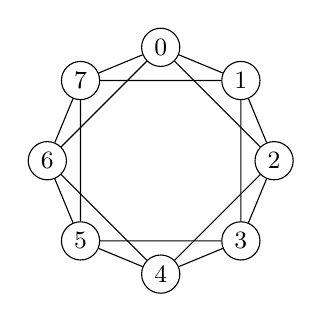
\begin{tikzpicture}[scale=1.2, every node/.style={circle,draw,inner sep=0.8mm, font=\small}]
            % H_{4,8} (a)
            \foreach \i in {0,...,7} {
                \node (\i) at (90-\i*45:1.2) {\i};
            }
            \foreach \i in {0,...,7} {
                \pgfmathtruncatemacro{\next}{mod(\i+1,8)}
                \pgfmathtruncatemacro{\skipone}{mod(\i+2,8)}
                \draw (\i) -- (\next);
                \draw (\i) -- (\skipone);
            }
        \end{tikzpicture}
        \\ (a)
    \end{minipage}
    \hfill
    \begin{minipage}{0.3\textwidth}
        \centering
        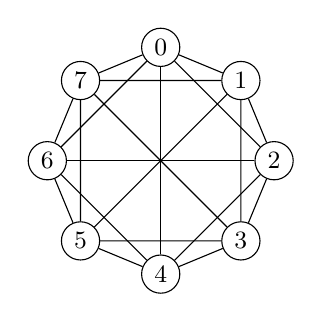
\begin{tikzpicture}[scale=1.2, every node/.style={circle,draw,inner sep=0.8mm, font=\small}]
            % H_{5,8} (b)
            \foreach \i in {0,...,7} {
                \node (\i) at (90-\i*45:1.2) {\i};
            }
            \foreach \i in {0,...,7} {
                \pgfmathtruncatemacro{\next}{mod(\i+1,8)}
                \pgfmathtruncatemacro{\skipone}{mod(\i+2,8)}
                \draw (\i) -- (\next);
                \draw (\i) -- (\skipone);
            }
            % Diametric edges for m=5
            \foreach \i in {0,1,2,3} {
                \pgfmathtruncatemacro{\opp}{\i+4}
                \draw (\i) -- (\opp);
            }
        \end{tikzpicture}
        \\ (b)
    \end{minipage}
    \hfill
    \begin{minipage}{0.3\textwidth}
        \centering
        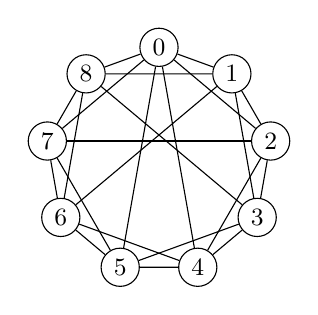
\begin{tikzpicture}[scale=1.2, every node/.style={circle,draw,inner sep=0.8mm, font=\small}]
            % H_{5,9} (c)
            \foreach \i in {0,...,8} {
                \node (\i) at (90-\i*40:1.2) {\i};
            }
            \foreach \i in {0,...,8} {
                \pgfmathtruncatemacro{\next}{mod(\i+1,9)}
                \pgfmathtruncatemacro{\skipone}{mod(\i+2,9)}
                \draw (\i) -- (\next);
                \draw (\i) -- (\skipone);
            }
            % Special edges for Case 3 (m odd, n odd)
            \draw (0) -- (4);
            \draw (0) -- (5);
            \draw (1) -- (6);
            \draw (2) -- (7);
            \draw (3) -- (8);
        \end{tikzpicture}
        \\ (c)
    \end{minipage}
    \caption{(a) $H_{4,8}$; (b) $H_{5,8}$; (c) $H_{5,9}$}
\end{figure}


\subsection{Whitney's Theorem and Ear Decompositions}

Whitney's Theorem provides a structural characterization of $2$-connected graphs, showing they can be built up from a simple cycle by adding "ears."

\begin{definition}[Ear]
An \emph{ear} of a graph $H$ is a path $P$ whose endpoints belong to $H$, but whose internal vertices (and edges) do not. 
\begin{itemize}
    \item If the endpoints of the path are distinct, it is an \textbf{open ear}.
    \item If the endpoints are the same vertex, it is a \textbf{closed ear} (a cycle attached at one point).
\end{itemize}
\end{definition}

\begin{theorem}[Whitney, 1932]
A graph $G$ is $2$-connected if and only if it has an \emph{ear decomposition}. That is, there exists a sequence of subgraphs $G_0, G_1, \dots, G_k = G$ such that:
\begin{enumerate}
    \item $G_0$ is a cycle.
    \item $G_{i+1}$ is obtained by adding an open ear to $G_i$ for all $0 \le i < k$.
\end{enumerate}
\end{theorem}

\noindent \textbf{Building a 2-connected Graph}\\
Start with a cycle $C_4$. By adding a path (ear) between two non-adjacent vertices, we create a graph that remains $2$-connected. If we added a "closed ear" (a loop at a single vertex), the graph would only be $1$-connected because that single vertex would become a cut-vertex.

\begin{figure}[H]
    \centering
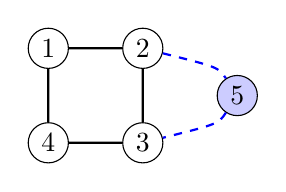
\begin{tikzpicture}[scale=1.2, every node/.style={circle,draw,inner sep=0.8mm}]
    % Base Cycle G0
    \node (1) at (0,1) {1};
    \node (2) at (1,1) {2};
    \node (3) at (1,0) {3};
    \node (4) at (0,0) {4};
    \draw[thick] (1) -- (2) -- (3) -- (4) -- (1);
    
    % The Ear (G1)
    \node[fill=blue!20] (5) at (2, 0.5) {5};
    \draw[thick, blue, dashed] (2) .. controls (1.8, 0.8) .. (5);
    \draw[thick, blue, dashed] (5) .. controls (1.8, 0.2) .. (3);

    \end{tikzpicture}
    \caption{Cycle $G_0$ with an added dashed blue \textbf{ear} ($G_1$)}
\end{figure}

\subsection{Intuition behind the Theorem}
The presence of an ear ensures that there are always at least two internally disjoint paths between any two vertices. 
\begin{itemize}
    \item In the base cycle, there are two paths between any two nodes.
    \item Adding an \emph{open} ear creates new paths without creating a "bottleneck" (cut-vertex).
    \item A \textbf{cut-vertex} only appears if we attach a piece of the graph to only one point; the ear decomposition prevents this by requiring two distinct attachment points.
\end{itemize}

\subsection{Summary of Chapter 3}

\begin{itemize}
    \item Vertex- and edge-connectivity measure robustness of graphs.
    \item Connectivity is bounded by minimum degree.
    \item Menger's Theorem links connectivity to disjoint paths.
    \item Blocks describe the $2$-connected structure of graphs.
    \item Block graphs form trees and provide a global decomposition.
    \item Connectivity theory underpins network reliability.
\end{itemize}
\clearpage

\section{Euler Tours and Hamilton Cycles}

\subsection{Walks, Trails, and Tours}

To understand Eulerian properties, we must distinguish between different ways of "moving" through a graph.

\begin{definition}[Trail and Closed Trail]
A \emph{trail} is a walk in which all edges are distinct (no edge is repeated).\\
A \emph{closed trail} is a trail that starts and ends at the same vertex.
\end{definition}

\begin{definition}[Euler Trail and Euler Tour]
Let $G$ be a graph.
\begin{itemize}
    \item An \textbf{Euler trail} is a trail that traverses every edge of $G$ exactly once.
    \item An \textbf{Euler tour} (or \emph{Euler circuit}) is a closed trail that traverses every edge of $G$ exactly once.
\end{itemize}
\end{definition}

\begin{figure}[H]
\centering
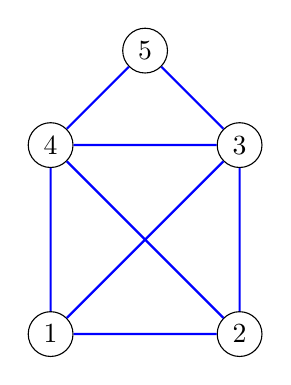
\begin{tikzpicture}[scale=1.2, every node/.style={circle,draw,inner sep=1mm}]
    % A classic Eulerian graph: The "Envelope" (without the bottom edge)
    \node (A) at (0,0) {1};
    \node (B) at (2,0) {2};
    \node (C) at (2,2) {3};
    \node (D) at (0,2) {4};
    \node (E) at (1,3) {5};
    \draw[thick, blue] (A) -- (B) -- (C) -- (D) -- (A) -- (C) -- (E) -- (D) -- (B);
    \end{tikzpicture}
    \caption{An Euler Tour: Every vertex has degree 2 or 4.}
\end{figure}
\clearpage

\subsection{Characterization of Eulerian Graphs}

\begin{definition}[Eulerian Graph]
A connected graph is \textbf{Eulerian} if it contains an Euler tour. 
\end{definition}

\begin{theorem}[Euler's Theorem, 1736]
A connected graph $G$ is Eulerian if and only if every vertex of $G$ has an \textbf{even degree}.
\end{theorem}

\noindent \textit{Intuition}
Whenever the tour enters a vertex via one edge, it must leave that vertex via a different, unused edge. Therefore, edges must come in pairs (one "in" and one "out"). This applies to every vertex, including the start/end vertex because the tour is closed.

\begin{theorem}[Euler Trail Condition]
A connected graph has an \textbf{Euler trail} (but no tour) if and only if it has \textbf{exactly two} vertices of odd degree. These two vertices will be the start and end points of the trail.
\end{theorem}



\noindent \textbf{Comparison of Common Graphs}
\begin{itemize}
    \item \textbf{Cycles ($C_n$):} Always Eulerian since every vertex has degree 2.
    \item \textbf{Complete Graphs ($K_n$):} $K_n$ is Eulerian if and only if $n$ is odd (so that each vertex has degree $n-1$, which is even).
    \item \textbf{Bipartite Graphs ($K_{r,s}$):} Eulerian if and only if both $r$ and $s$ are even.
\end{itemize}

\subsection{The Seven Bridges of K\"onigsberg}
The study of graph theory began with this problem. The city had seven bridges. Representing landmasses as vertices and bridges as edges, the resulting multigraph had four vertices with odd degrees ($3, 3, 3,$ and $5$). Since more than two vertices had odd degrees, Euler proved it was impossible to cross every bridge exactly once and return to the start.

\subsection{Algorithm for Finding Euler Tours}

While Fleury's Algorithm is another option, \textbf{Hierholzer's Algorithm} is generally preferred for its efficiency ($O(E)$ time complexity).

\begin{algorithm}[Hierholzer's Algorithm]
Given a connected graph $G$ where all vertices have even degree:
\begin{enumerate}
    \item \textbf{Initial Circuit:} Start at any vertex $v$. Follow unused edges until you return to $v$. Since all degrees are even, you are guaranteed never to get "stuck" at a vertex other than the start. Label this circuit $C$.
    \item \textbf{Find Sub-circuits:} If there are edges in $G$ not in $C$, pick a vertex $u$ belonging to $C$ that is incident to an unused edge. Start a new trail from $u$, again following unused edges until returning to $u$.
    \item \textbf{Splicing:} Integrate the new sub-circuit into the original circuit $C$ at vertex $u$.
    \item \textbf{Repeat:} Continue until all edges are included in the tour.
\end{enumerate}
\end{algorithm}

\begin{algorithm}[Fleury's Algorithm]
This algorithm builds a single path by following one rule: \textbf{Never cross a bridge unless you have no other choice.}
\begin{enumerate}
    \item Start at any vertex $v$.
    \item At each step, choose an unused edge incident to the current vertex such that its removal does not disconnect the graph of remaining edges (i.e., do not pick a bridge of the remaining subgraph).
    \item If only a bridge is available, you must take it.
    \item Terminate when all edges have been traversed.
\end{enumerate}
\end{algorithm}

\subsection{Comparison of Algorithms}

While both algorithms are mathematically sound, they serve different purposes:

\begin{table}[H]
\centering
\begin{tabular}{lll}
\hline
\textbf{Feature} & \textbf{Hierholzer's} & \textbf{Fleury's} \\ \hline
\textbf{Strategy} & Splicing cycles together & Extending a single trail \\
\textbf{Complexity} & $O(E)$ (Linear) & $O(E^2)$ (due to bridge testing) \\
\textbf{Use Case} & Computer implementations & Manual/human solving \\
\textbf{Philosophy} & Modular construction & Greedy with foresight \\ \hline
\end{tabular}
\end{table}

\noindent \textbf{Applying Fleury's Rule}\\
Imagine a graph shaped like a figure-8 (two triangles joined at a single vertex $v$). If you start at $v$ and traverse one triangle, the last edge you use to return to $v$ becomes a bridge to the second triangle. Fleury's rule ensures you finish the first triangle completely before "crossing over" to the second.

\begin{figure}[H]
\centering
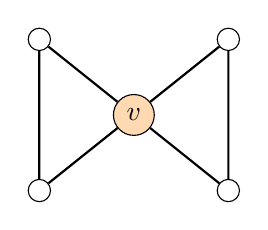
\begin{tikzpicture}[scale=1.2, every node/.style={circle,draw,inner sep=1mm}]
    \node (1) at (-1, 0.8) {};
    \node (2) at (-1, -0.8) {};
    \node[fill=orange!30] (V) at (0, 0) {$v$};
    \node (3) at (1, 0.8) {};
    \node (4) at (1, -0.8) {};

    \draw[thick] (1) -- (2) -- (V) -- (1);
    \draw[thick] (V) -- (3) -- (4) -- (V);
\end{tikzpicture}
    \caption{In a Figure-8, $v$ is the critical "pivot" for Fleury's Rule.}
\end{figure}


\subsection{Applications: The Chinese Postman Problem (CPP)}

The \textbf{Route Inspection Problem}, popularly known as the Chinese Postman Problem (coined by Jack Edmonds in honor of Mei-Ko Kwan), asks for the shortest path that covers every edge.

\begin{problem}[The CPP Challenge]
If a graph is Eulerian, any Euler tour is an optimal solution. However, if the graph has $2k$ vertices of odd degree, some edges \textit{must} be traversed more than once. The goal is to choose these "duplicated" edges such that their total weight is minimized.
\end{problem}
\clearpage

\begin{theorem}[Optimal Strategy]
To solve the CPP on a non-Eulerian graph:
\begin{enumerate}
    \item Identify all vertices with \textbf{odd degree}. (There will always be an even number of them).
    \item Find a \textbf{minimum weight matching} between these odd-degree vertices. This involves finding paths between pairs of odd vertices such that the sum of the path weights is minimized.
    \item "Duplicate" the edges along these shortest paths. This effectively makes every vertex have an even degree.
    \item Find an Euler tour in this new augmented graph.
\end{enumerate}
\end{theorem}

\subsubsection{Postman on a Non-Eulerian Grid}
Imagine a rectangular grid where only the four corner vertices have degree 2 and the rest have degree 3 or 4.
\begin{itemize}
    \item \textbf{Odd Vertices:} Identify the "dead ends" or intersections with 3 streets.
    \item \textbf{Edge Duplication:} A postman might have to walk down "Main Street" twice to return to the depot after visiting a dead-end alley.
\end{itemize}

\begin{figure}[H]
\centering
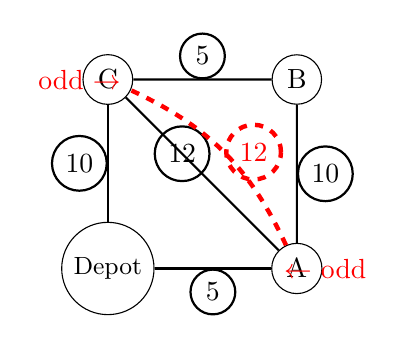
\begin{tikzpicture}[scale=1.2, every node/.style={circle,draw,inner sep=1mm}]
    \node (D) at (0,0) {\small Depot};
    \node (A) at (2,0) {A};
    \node (B) at (2,2) {B};
    \node (C) at (0,2) {C};

    % Original Edges
    \draw[thick] (D) -- (A) node[midway, below] {5};
    \draw[thick] (A) -- (B) node[midway, right] {10};
    \draw[thick] (B) -- (C) node[midway, above] {5};
    \draw[thick] (C) -- (D) node[midway, left] {10};
    \draw[thick] (A) -- (C) node[midway, above left] {12};
    
    % Indicators of odd degree
    \node[draw=none, red] at (2.3,0) {$\leftarrow$ odd};
    \node[draw=none, red] at (-0.3,2) {odd $\rightarrow$};

    % Duplicated edge (the solution to CPP)
    \draw[dashed, red, ultra thick, bend right=20] (A) to node[midway, right] {12} (C);
\end{tikzpicture}
\caption{In the example above, the postman duplicates the edge $AC$ (weight 12) to make the graph Eulerian.}
\end{figure}

\subsection{Hamilton Paths and Cycles}

While Eulerian properties focus on traversing every \textbf{edge}, Hamiltonian properties focus on visiting every \textbf{vertex}. Interestingly, while checking if a graph is Eulerian is easy ($O(E)$), checking if a graph is Hamiltonian is an NP-complete problem.

\begin{definition}[Hamilton Path and Hamilton Cycle]
Let $G$ be a graph.
\begin{itemize}
    \item A \textbf{Hamilton path} is a path that visits every vertex in $G$ exactly once.
    \item A \textbf{Hamilton cycle} is a cycle that visits every vertex in $G$ exactly once.
\end{itemize}
\end{definition}

\begin{definition}[Hamiltonian Graph]
A graph is \textbf{Hamiltonian} if it contains at least one Hamilton cycle.
\end{definition}

\begin{figure}[H]
\centering
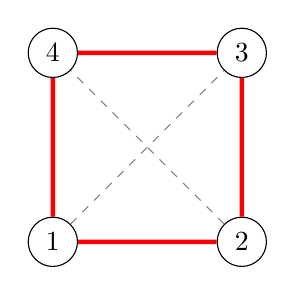
\begin{tikzpicture}[scale=1.2, every node/.style={circle,draw,inner sep=1.2mm}]
    % C4 with diagonals
    \node (1) at (0,0) {1};
    \node (2) at (2,0) {2};
    \node (3) at (2,2) {3};
    \node (4) at (0,2) {4};

    % Hamilton cycle highlighted
    \draw[ultra thick, red] (1) -- (2) -- (3) -- (4) -- (1);
    
    % Additional edges to show it's not just a cycle
    \draw[gray, dashed] (1) -- (3);
    \draw[gray, dashed] (2) -- (4);
\end{tikzpicture}
\caption{Red cycle visits all vertices exactly once.}
\end{figure}

\subsection{Sufficient Conditions for Hamiltonicity}

Since finding a Hamilton cycle is hard, we rely on \textbf{sufficient conditions}—rules that say "if the graph is dense enough, it must be Hamiltonian." Note that these are not \textit{necessary}; a graph can be Hamiltonian without meeting these criteria.

\begin{theorem}[Dirac's Theorem, 1952]
Let $G$ be a simple graph with $n \ge 3$ vertices. If every vertex has a degree of at least $n/2$:
\[ \delta(G) \ge \frac{n}{2} \]
then $G$ is Hamiltonian.
\end{theorem}

\begin{theorem}[Ore's Theorem, 1960]
Let $G$ be a simple graph with $n \ge 3$ vertices. If for every pair of non-adjacent vertices $u$ and $v$:
\[ \text{deg}(u) + \text{deg}(v) \ge n \]
then $G$ is Hamiltonian. (Note: Dirac's Theorem is a special case of Ore's).
\end{theorem}

\noindent Hamiltonian vs. Non-Hamiltonian
\begin{itemize}
    \item \textbf{Complete Graphs ($K_n$):} Always Hamiltonian for $n \ge 3$.
    \item \textbf{Cycles ($C_n$):} Always Hamiltonian by definition.
    \item \textbf{Petersen Graph:} This is a famous example of a graph that is \textbf{not} Hamiltonian, even though it is highly symmetrical and 3-regular.
    \item \textbf{Bipartite Graphs ($K_{m,n}$):} Hamiltonian only if $m = n$. If the sets are unequal, you will eventually get "stuck" in the larger set.
\end{itemize}

\subsubsection{Famous Examples: Hamiltonian and Non-Hamiltonian Graphs}

The Petersen graph is perhaps the most famous graph in this context. It is 3-regular, 3-connected, and has 10 vertices, yet it is \textbf{not Hamiltonian}. It does, however, contain a Hamilton path.

The dodecahedron graph represents the edges and vertices of a dodecahedron. Unlike the Petersen graph, the dodecahedron \textbf{is Hamiltonian}.


\subsection{Summary: Euler vs. Hamilton}
\begin{table}[h]
\centering
\begin{tabular}{lll}
\hline
\textbf{Feature} & \textbf{Eulerian} & \textbf{Hamiltonian} \\ \hline
\textbf{Requirement} & Visit every \textbf{edge} once & Visit every \textbf{vertex} once \\
\textbf{Key Criteria} & Even degrees & Graph density (Dirac/Ore) \\
\textbf{Complexity} & $P$ (Easy to solve) & $NP$-Complete (Hard to solve) \\ \hline
\end{tabular}
\end{table}
\clearpage

\subsection{Closure of a Graph}

The concept of a closure allows us to simplify a graph while preserving its "Hamiltonian nature." It essentially fills in the "obvious" edges that don't change whether a Hamilton cycle exists.

\begin{definition}[Closure]
The \emph{closure} of a graph $G$, denoted $\text{cl}(G)$, is the graph obtained from $G$ by recursively joining pairs of non-adjacent vertices $u, v$ whose degree sum satisfies:
\[ d(u) + d(v) \ge n \]
where $n = |V(G)|$. This process continues until no such pair of vertices remains.
\end{definition}

\begin{theorem}[Bondy--Chv\'atal Theorem, 1976]
A graph $G$ is Hamiltonian if and only if its closure $\text{cl}(G)$ is Hamiltonian.
\end{theorem}

\begin{corollary}
If the closure of a graph $G$ is a complete graph $K_n$, then $G$ is Hamiltonian. This provides a much stronger condition than Ore's Theorem.
\end{corollary}

\subsection{The Travelling Salesman Problem (TSP)}

While the Hamilton Cycle problem asks "Can we visit every city?", the \textbf{Travelling Salesman Problem} asks "What is the cheapest way to visit every city and return home?"

\begin{problem}[Travelling Salesman Problem]
Given a complete graph $K_n$ where each edge $e$ has a weight $w(e)$, find a Hamilton cycle $C$ such that the total weight $\sum_{e \in C} w(e)$ is minimized.
\end{problem}

Unlike the Chinese Postman Problem (which is $P$), the TSP is \textbf{NP-hard}. As $n$ increases, the number of possible cycles $(n-1)!/2$ grows factorially, making brute-force search impossible for large networks.

\subsubsection{Metric TSP and the Triangle Inequality}
In many real-world applications, the weights satisfy the \textbf{Triangle Inequality}:
\[ w(u,v) \le w(u,x) + w(x,v) \]
This means a direct flight is never more expensive than a layover. For "Metric TSP," we can find approximate solutions (like the Double Tree Algorithm) that are guaranteed to be within a certain factor of the true optimum.

\noindent \textbf{Real-World Modeling}
\begin{itemize}
    \item \textbf{Logistics:} Minimizing fuel consumption for delivery trucks.
    \item \textbf{Manufacturing:} A robotic drill must visit 1,000 hole locations on a circuit board in the shortest time possible.
    \item \textbf{Genetics:} Reconstructing DNA sequences by finding the shortest overlap between fragments.
\end{itemize}

%========================
% Improved TikZ: Weighted TSP
%========================
\begin{figure}[H]
\centering
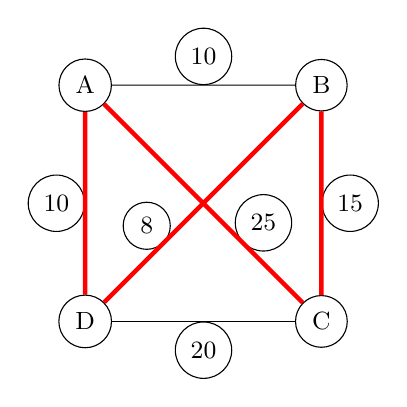
\begin{tikzpicture}[scale=1.5, every node/.style={circle,draw,inner sep=1.2mm, font=\small}]
    \node (A) at (0,2) {A};
    \node (B) at (2,2) {B};
    \node (C) at (2,0) {C};
    \node (D) at (0,0) {D};

    % Edges with weights
    \draw (A) -- (B) node[midway, above] {10};
    \draw (B) -- (C) node[midway, right] {15};
    \draw (C) -- (D) node[midway, below] {20};
    \draw (D) -- (A) node[midway, left] {10};
    \draw (A) -- (C) node[midway, above right, pos=0.7] {25};
    \draw (B) -- (D) node[midway, above left, pos=0.7] {8};

    % Highlighted Optimal Hamilton Cycle: A-B-C-D-A = 55, A-B-D-C-A = 10+8+20+25 = 63, A-D-B-C-A = 10+8+15+25 = 58
    % Let's highlight A-D-B-C-A or similar
    \draw[ultra thick, red] (A) -- (D) -- (B) -- (C) -- (A);
\end{tikzpicture}
\caption{Optimal Route: $10+8+15+25 = 58$}
\end{figure}
\clearpage

\subsubsection{Case Studies: The Petersen, Dodecahedron, and Herschel Graphs}

\textbf{The Petersen Graph}

\noindent The Petersen graph is a 3-regular (cubic) graph with 10 vertices and 15 edges. It is famously \textbf{non-Hamiltonian}, making it the most prominent counterexample to many early conjectures about symmetrical, highly-connected graphs. Despite having no Hamilton cycle, it is 3-connected and contains a Hamilton path between any two vertices.

\begin{figure}[H]
\centering
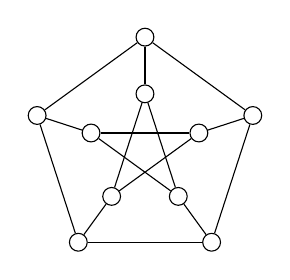
\begin{tikzpicture}[scale=1.2, every node/.style={circle,draw,inner sep=0.8mm}]
    % Outer pentagon
    \foreach \i in {0,...,4} {
        \node (o\i) at ({90-\i*72}:1.2) {};
        \node (i\i) at ({90-\i*72}:0.6) {};
    }
    % Edges
    \foreach \i in {0,...,4} {
        \pgfmathtruncatemacro{\next}{mod(\i+1,5)}
        \pgfmathtruncatemacro{\star}{mod(\i+2,5)}
        \draw (o\i) -- (o\next);
        \draw (i\i) -- (i\star);
        \draw (o\i) -- (i\i);
    }
\end{tikzpicture}
\caption{The Petersen Graph: Symmetrical but non-Hamiltonian.}
\end{figure}

\noindent\textbf{Dodecahedron and Herschel Graphs}

\noindent While both are 3-connected and planar, these two graphs differ fundamentally in their Hamiltonicity. The Dodecahedron is the classic example of a Hamiltonian polyhedral graph, while the Herschel graph is the smallest polyhedral graph that is non-Hamiltonian.

\begin{figure}[H]
    \centering
    % --- (a) The Dodecahedron ---
    \begin{minipage}{0.48\textwidth}
        \centering
        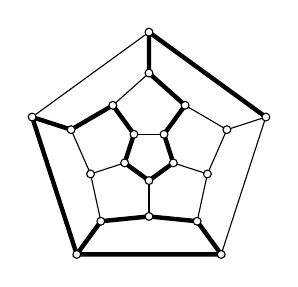
\begin{tikzpicture}[scale=1.3, every node/.style={circle, draw, fill=white, inner sep=1pt}]
            \foreach \i in {0,...,4} {
                \coordinate (outer\i) at ({18 + \i*72}:1.2);
                \coordinate (mid\i)   at ({18 + \i*72}:0.8);
                \coordinate (inner\i) at ({54 + \i*72}:0.6);
                \coordinate (core\i)  at ({54 + \i*72}:0.25);
            }
            \foreach \i in {0,...,4} {
                \pgfmathtruncatemacro{\next}{mod(\i+1, 5)}
                \pgfmathtruncatemacro{\prev}{mod(\i+4, 5)}
                \draw (outer\i) -- (outer\next);
                \draw (outer\i) -- (mid\i);
                \draw (mid\i) -- (inner\i);
                \draw (mid\i) -- (inner\prev);
                \draw (inner\i) -- (core\i);
                \draw (core\i) -- (core\next);
            }
            % Example Hamilton Cycle in bold
            \draw[ultra thick] (outer0) -- (outer1) -- (mid1) -- (inner0) -- (core0) -- (core4) -- (core3) -- (core2) -- (core1) -- (inner1) -- (mid2) -- (outer2) -- (outer3) -- (outer4) -- (mid4) -- (inner3) -- (mid3) -- (outer3) -- (outer4); 
            \foreach \i in {0,...,4} {
                \node at (outer\i) {}; \node at (mid\i) {};
                \node at (inner\i) {}; \node at (core\i) {};
            }
        \end{tikzpicture}
    \end{minipage}
    \hfill
    % --- (b) The Herschel Graph ---
    \begin{minipage}{0.48\textwidth}
        \centering
        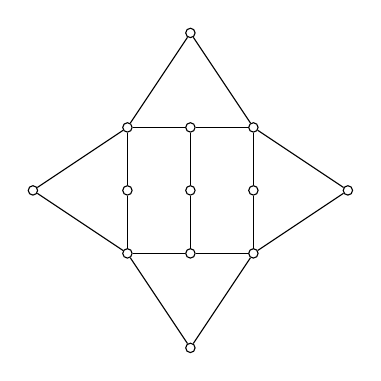
\begin{tikzpicture}[scale=1, every node/.style={circle, draw, fill=white, inner sep=1.2pt}]
            \node (top) at (0,2) {};
            \node (bottom) at (0,-2) {};
            \node (left) at (-2,0) {};
            \node (right) at (2,0) {};
            \node (center) at (0,0) {};
            \node (it) at (0,0.8) {}; \node (ib) at (0,-0.8) {};
            \node (il) at (-0.8,0) {}; \node (ir) at (0.8,0) {};
            \node (ml) at (-0.8,0.8) {}; \node (mr) at (0.8,0.8) {};
            \node (mbl) at (-0.8,-0.8) {}; \node (mbr) at (0.8,-0.8) {};

            \draw (top) -- (ml) -- (left) -- (mbl) -- (bottom) -- (mbr) -- (right) -- (mr) -- (top);
            \draw (ml) -- (it) -- (mr) (mbl) -- (ib) -- (mbr);
            \draw (it) -- (center) -- (ib) (ml) -- (il) -- (mbl) (mr) -- (ir) -- (mbr);
        \end{tikzpicture}
    \end{minipage}
    \caption{The Dodecahedron \small Hamiltonian (20 vertices) - The Herschel Graph \small Non-Hamiltonian (11 vertices)}
\end{figure}

\end{document}
